\section{Analog Feedback and MCU Inputs}
\label{sec:hw-sensing}

On the V1.0 test platform, the controller acquires scaled primary voltage at PA0, isolated secondary-bulk voltage at PA1, and the LMG2652 half-bridge-current signal at PA2. TLV9064 buffers reduce ADC loading of the sensing circuits. The AMC0330 transfers secondary-voltage feedback across the isolation barrier to the primary-side MCU. V2 uses the same measurements with direct ADC connections, as shown in \Cref{fig:schematic-mcu}.

\begin{figure}[htbp]
\centering
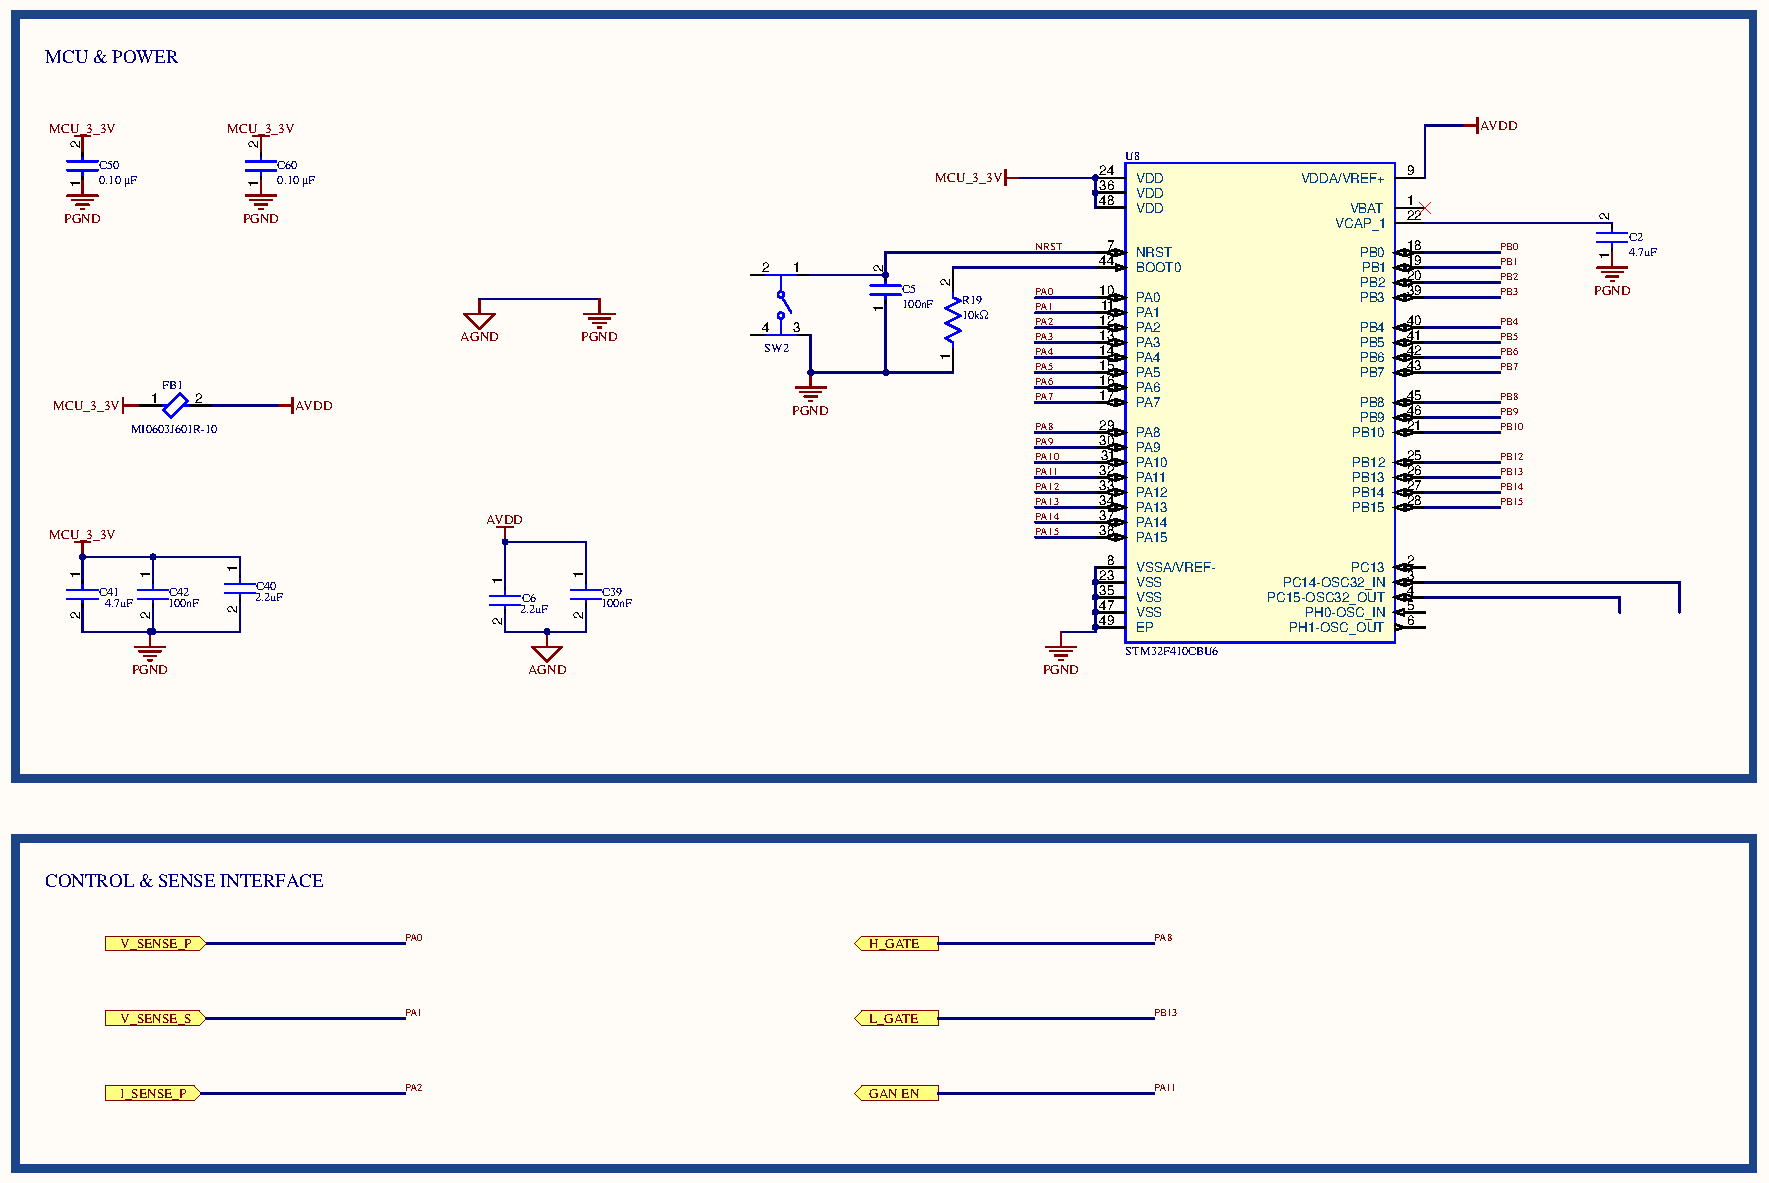
\includegraphics[width=\textwidth,height=0.57\textheight,keepaspectratio]{Pictures/Thesis/07_Hardware/Rebuilt/schematic_v2_controller_excerpt.pdf}
\caption{V2 sheet 4 MCU connections. Feedback enters pins PA0--PA2 directly; PA8/PB13 provide carrier commands and PA11 provides burst enable. The MCU uses the primary-side ground reference.}
\label{fig:schematic-mcu}
\end{figure}

\begin{table}[htbp]
\centering
\caption{MCU feedback pins and their functions.}
\label{tab:hw-sensing-evidence}
\begin{tabularx}{\textwidth}{@{}p{0.12\textwidth}p{0.32\textwidth}X@{}}
\toprule
MCU pin & Input & Firmware function\\
\midrule
PA0 & Primary-voltage feedback & Diagnostics and optional high-line duty reduction\\
PA1 & Isolated secondary-bulk voltage & Voltage regulation and overvoltage protection\\
PA2 & Half-bridge current sensing & Load detection, diagnostics, and optional current protection\\
\bottomrule
\end{tabularx}
\end{table}

The half-bridge-current signal at PA2 was used for load classification. Its product with secondary voltage at PA1 does not represent connector output power without a validated conversion model. Output power was therefore calculated from external VBUS and load-current measurements, while the controller regulated secondary-bulk voltage.

V1.0 includes an external \SI{2.5}{\volt} reference, omitted in V1.1, while the final firmware defaults to a \SI{3.3}{\volt} ADC reference. Divider ratios, amplifier scale, buffers, gain, and offset also affect the conversion, so the scales must be checked against measured circuit and ADC-pin voltages. The calibration settings are given in \Cref{sec:ctrl-feedback}.
